\section{Systemmodelle}

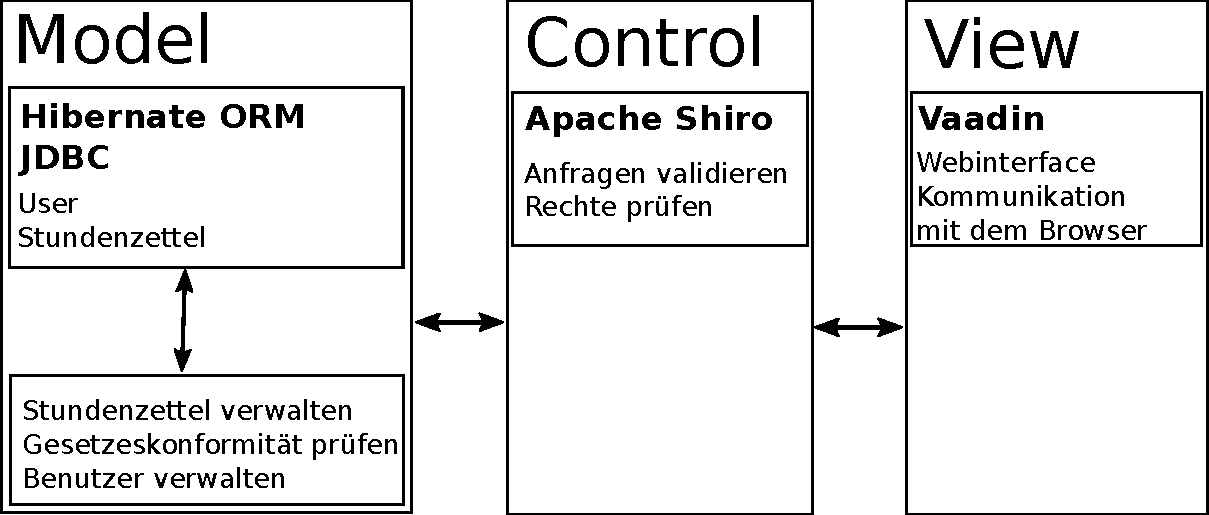
\includegraphics[width=\linewidth]{mvc.pdf}\\
\\
Die Architektur der Software basiert auf dem Model-View-Control (MVC) Modell, welches eine strikte Trennung von Daten/Logik (Model), Oberfläche (View) und Steuerung (Control) vorsieht.
Dies verbessert zum einen die Wartbarkeit und vereinfacht den Austausch einzelner Module, vor allem der Oberfläche.
\begin{itemize}
	\item \textbf{Model:}
		Das Model enthält die Benutzer und Stundenzettel.
		Es enthält die Funktionalität um Benutzer und Stundenzettel zu verwalten.
		Außerdem prüft es, ob die Stundenzettel den gesetzlichen Regelungen entsprechen und leitet sonst entsprechende Maßnahmen ein.
	\item \textbf{View:}
		Das View zeigt dem Benutzer alle Funktionalitäten und Informationen an, die für diesen relevant sind.
		Zudem nimmt es Befehle desselbigen entgegen.
		Es ist die Schnittstelle über die alle Interaktion mit dem Benutzer passiert.
	\item \textbf{Control:}
		Das Control prüft alle Anfragen die es vom View bekommt auf Korrektheit.
		Zudem prüft es ob der entsprechende Benutzer die nötigen Rechte für die Anfrage hat.
		Dann leitet es die Anfrage gegebenenfalls an das Model weiter.
\end{itemize}
